\chapter{Results}
\label{chap:results}

\section{Software engineering}

\subsection{Student tasks}
\label{subsec:studenttasks}
In order to find potential and noteworthy differences between the tasks of postgraduate students and undergraduate students a questionnaire was made. The questionnaire was also aimed at finding how much these students are using task management applications such as to-do lists or calendars, both in terms of regularity and frequency. The questionnaire yielded 105 responses where 62.9\% of these were Bachelor degree students. The remaining 37.1\% were Master or PhD students. This was determined by the first question in the questionnaire.

We also wanted to know whether or not these students typically make lists of the things that they have to do. The students were asked to reply to the following statement: \emph{I make a list of the things I have to do during a day/week}. Possible responses to the statement were: \emph{Never}, \emph{1-2 times per week}, \emph{Almost every day} and \emph{Every day, multiple times}. The responses among all students are shown in Figure~\ref{fig:todolistusage}.
\begin{figure}[tbp]
  \centering
  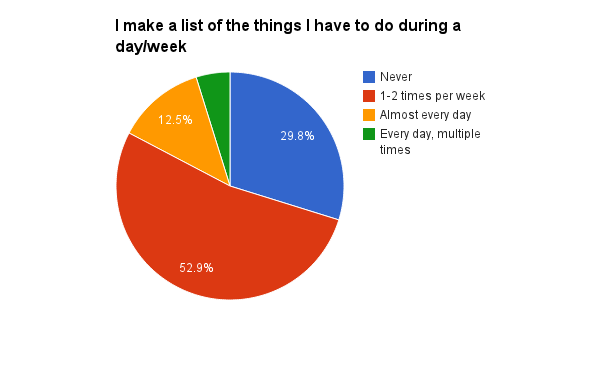
\includegraphics[width=\textwidth]{figures/TodoListUsage.png}
  \caption[To-do list usage]{The distribution of how often students make to-do lists.}
  \label{fig:todolistusage}
\end{figure}

We also wanted to get an overview over the amount of students who were using task management applications at all. For this, we asked the question \emph{Do you use task/time management applications such as calendars or to-do lists?}. 64.8\% replied \emph{Yes}, while the remaining 35.2\% replied \emph{No}.

An important part of the questionnaire was to find out the regularity at which students do certain type of tasks. For this, we listed the predefined tasks and asked the students to reply on a scale of how regular they did the tasks. The question were \emph{How regular do you perform the following tasks?} The scale that was used in this case consisted of \emph{Every day}, \emph{Every week}, \emph{Every month}, \emph{Irregular, zero or few times per week} and \emph{Irregular, zero or few times per month}. This question can let us know what kind of tasks are done on a regular basis and what tasks are done more randomly. The responses are shown in Figure~\ref{fig:taskregularity}
\begin{figure}[tbp]
  \centering
  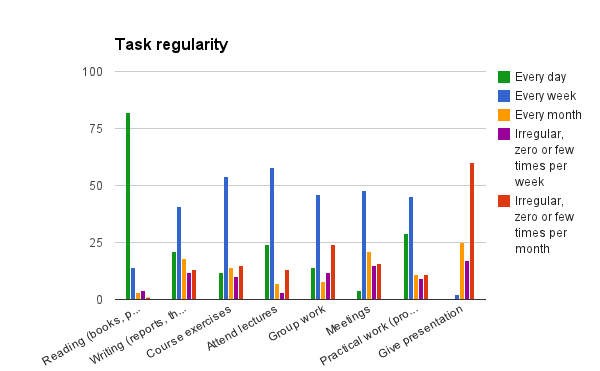
\includegraphics[width=\textwidth]{figures/TaskRegularity.png}
  \caption[Student task regularity]{The distribution of how regular particular tasks are done.}
  \label{fig:taskregularity}
\end{figure}

A very similar question was formed to provide feedback on how often the different tasks were being done. On the question \emph{On average, how often do you perform the following tasks?} the students were asked to reply on a scale for each of the predefined tasks. The scale consisted of \emph{Less than once per week}, \emph{1-2 times per week}, \emph{3-4 times per week}, \emph{About once per day} and \emph{Multiple times per day}. Responses to this question are shown in Figure~\ref{fig:taskfrequency}.
\begin{figure}[tbp]
  \centering
  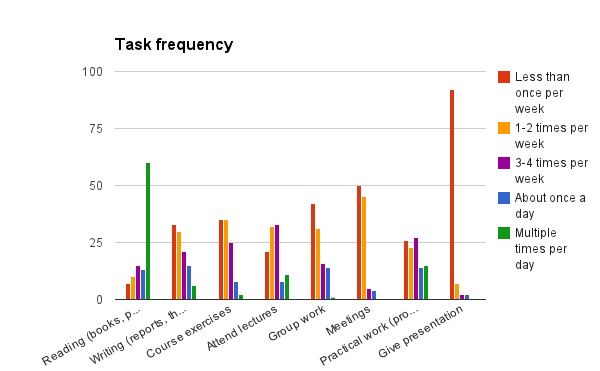
\includegraphics[width=\textwidth]{figures/TaskFrequency.png}
  \caption[Student task frequency]{The distribution of how often (frequent) particular tasks are done.}
  \label{fig:taskfrequency}
\end{figure}

In order to find out whether our predefined tasks were enough to cover all the tasks that a student typically does, we devised another question where the students were to input any other tasks that they typically did. The question and the responses are shown in Table~\ref{tab:othertasksresponses}
\begin{table}[tbp]
  \centering
  \begin{tabular}{|l|r|}
	\hline
	\textbf{Task} & \textbf{Frequency} \\
	\hline
	Reddit & All the time \\
  \hline
	Carry out experiment & Once a month \\
	\hline
	Part-time job (4) & 35"\%" \\
	\hline
	Searching for articles (2) &  \\
	\hline
	Gaming & \\
	\hline
	Workout/exercise & 4-5 times a week \\
	\hline
  \end{tabular}
  \caption[Other student tasks response]{Responses to the question \emph{What other tasks that were not previously mentioned do you do, and how often?} The number in parenthesis shows how many students responded the same thing.}
  \label{tab:othertasksresponses}
\end{table}


\subsection{Collected student tasks}
\label{subsec:collectedtasks}

From the application user experimenting at the end of the thesis, a total of 46 tasks were logged in the external database. This is too few to make any strong conclusions upon the data, but it might be possible to make some small indications. The distribution of the types of tasks that the students actually did is shown in Figure~\ref{fig:taskdistribution}.
\begin{figure}[tbp]
  \centering
  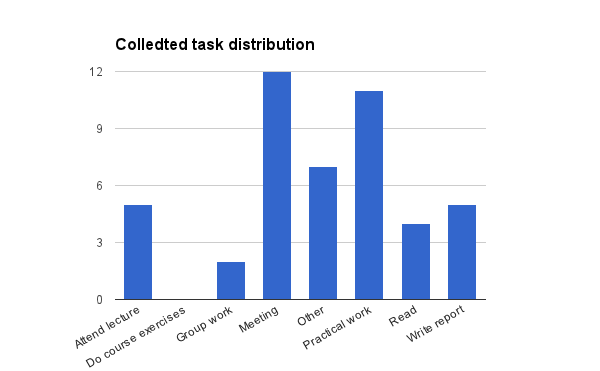
\includegraphics[width=\textwidth]{figures/TaskDistribution.png}
  \caption[Collected task type distribution]{The distribution of the types of tasks among the tasks that were collected.}
  \label{fig:taskdistribution}
\end{figure}
This shows that \emph{Meeting} was the type of task that were logged the most in the usage of the application, with 12 tasks being of this type. This might indicate that users typically log important tasks that they need to remember, and is therefore using the task entry as a reminder for the meeting.

Since we used a very limited set of predefined tasks, it would seem logical that the type \emph{Other} would receive a large share of the total amount of tasks. Although the intended usage was in an educational environment, this is not something that was controlled during the application usage experiment. It is then likely that some students would use the application for purposes other than just educational ones. However, only 7 (15\%) of the tasks were categorized as \emph{Other}. This would indicate that most of the student actually used the application for educational purposes.

The indications that the students were using the application as a reminder of events is further strengthened by looking at the tasks that were created with specific start and end times. Tasks or events that has a specific starting time is generally something that we need to remember. Of the 46 total tasks that were logged, 24 (52\%) of these were logged with both a starting time and an end time.

There are also a few other things that are interesting to look at. One is whether or not the users actually ``ticked'' or ``checked'' the tasks after completion as to indicate that the task is done. We could also check the amount of time spent on the different tasks, which would be available for the tasks that were actually tracked in the application.

Few of the tasks were ticked off as to indicate that they were finished. Of the 46 tasks, only 12 (26\%) were said to be completed in the application. The students probably completed more of the tasks than this would suggest, so it is likely that they simply forgot or chose not to ``tick off'' the task in the application.

Very few tasks were tracked with actual contexts in the application. Only 13 (28\%) had actual contexts related to them. The task categories that were tracked and the average time spent on these tasks is shown in Table~\ref{tab:avgtimespent}.
\begin{table}[tbp]
  \centering
  \begin{tabular}{|l|r|r|}
	\hline
	\textbf{Task category} & \textbf{Number of tracked tasks} & \textbf{Average time spent (minutes)} \\
	\hline
	Attend lecture & 1 & 62.1 \\
  \hline
	Do course exercises & 0 & 0 \\
  \hline
	Group work & 0 & 0 \\
  \hline
	Meeting & 3 & 81.7 \\
  \hline
	Other & 2 & 29.4 \\
  \hline
	Practical work & 3 & 152.2 \\
  \hline
	Read & 2 & 31.4 \\
  \hline
  Write report & 2 & 81.9 \\
  \hline
  \end{tabular}
  \caption[Time spent on tasks]{Number of tracked tasks in each category and the average time spent on those tasks.}
  \label{tab:avgtimespent}
\end{table}
We can see that the distribution of the task categories for the tasks that have been tracked with contexts are quite similar to the distribution of all the tasks registered in the application (see Figure~\ref{fig:taskdistributioncomparison}).
\begin{figure}[tbp]
  \centering
  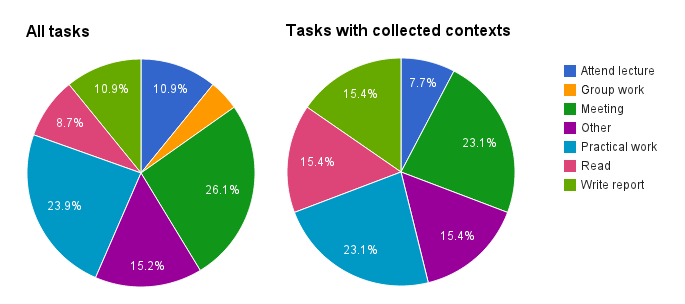
\includegraphics[width=\textwidth]{figures/TaskDistributionComparison.png}
  \caption[All tasks and tasks with collected contexts comparison]{The distribution of the types of tasks among all registered tasks and the ones with collected contexts.}
  \label{fig:taskdistributioncomparison}
\end{figure}

\subsection{Design decisions}


- Even simpler GUI for experiment.

\paragraph{sad}
Some sub sub 


\section{Context collection}

Looking at the data collected from the users tasks in Section~\ref{subsec:collectedtasks}, we can see that few tasks have been logged with an actual ``time spent'' value. The tasks that do not have this value, are tasks that have not been logged with contexts. This is because the users did not press the in-app start button, which means that they either forgot to do so, or that they ignored that part of the intended work flow. This is an indication that having users tracking their own tasks in this manner opens for inconsistencies and inaccuracies in the logging. It is hard for users to remember to log a task prior to the execution of the task.


Another thing is to see if the actual location that the users performed their tasks coincides with the planned location of the tasks.


\section{Domain}

